\documentclass[aip,jcp,reprint,showkeys]{revtex4-1}

\usepackage{graphicx,bm,xcolor,hyperref,amsmath,amssymb,amsfonts,float}
\usepackage{hyperref}
\usepackage{algorithmicx}
\usepackage{algcompatible}
\usepackage{algpseudocode} 
\newcommand{\LeftComment}[1]{\State {\scriptsize /* \textit{#1} */}}

\usepackage{tikz,tikzscale}

\newcommand{\alert}[1]{\textcolor{red}{#1}}
\newcommand{\ket}[1]{|#1\rangle}
\newcommand{\stwo}{\hat{S}^2}
\newcommand{\tu}{\mathtt{u}}
\newcommand{\ttt}{\mathtt{t}}
\newcommand{\mb}{\mathtt{b}}
\newcommand{\md}{\mathtt{d}}
\newcommand{\mD}{\mathcal{D}}
\newcommand{\mpp}{\mathtt{p}}
\newcommand{\mpv}{\mathbf{p}}
\newcommand{\up}{\uparrow}
\newcommand{\dn}{\downarrow}
\newcommand{\Nint}{{N_\text{int}}}
\newcommand{\Norb}{{N_\text{orb}}}
\newcommand{\one}{{\texttt{1}}}
\newcommand{\zero}{{\texttt{0}}}

\newcommand{\sop}{\textsc{sop}}
\newcommand{\cipsi}{\textsc{cipsi}}
\newcommand{\csf}{\textsc{csf}}
\newcommand{\mel}[3]{\langle #1 | #2 | #3 \rangle}
\newcommand{\ept}{E_\text{PT2}}




\begin{document}

\title{Enforcing spin adaptation in determinant-based selected configuration
interaction}

\author{Thomas Applencourt}
\affiliation{Argonne Leadership Computing Facility, Argonne National Laboratory, Argonne, Illinois 60439 USA}
\author{Kevin Gasperich}
\affiliation{Computational Science Division, Argonne National Laboratory, Argonne, Illinois 60439 USA}
\affiliation{Department of Chemistry, University of Pittsburgh, Pittsburgh, Pennsylvania 15260 USA}
\author{Anthony Scemama}
\affiliation{Laboratoire de Chimie et Physique Quantiques, Universit\'e de Toulouse, CNRS, UPS, France}

%%%%%%%%%%%%%%%%%%%%%%%%%%%%%%%%%%%%%%%%%%%%%%%%%%%%%%%%%%%%%%%%%
\begin{abstract}
We present an algorithm which, given an arbitrary determinant space, generates
all the missing determinants allowing one to obtain spin adapted wave
functions while avoiding working with configuration state functions.  Although
the idea to enforce spin adaptation in determinant-based calculations is not
new, we propose an original algorithm for the generation of the Slater
determinants which is extremely efficient: generating all the possible
determinants with 6 $\up$-spin and 6 $\dn$-spin electrons in 12 open shells
took 21 CPU cycles per generated Slater determinant. We also propose a
modification of the denominators in the Epstein-Nesbet perturbation theory
reducing significantly the non-invariance of the second order correction with
respect to different values of the spin quantum number $m_s$.  The
computational cost of this correction is also negligible.
\end{abstract}
%%%%%%%%%%%%%%%%%%%%%%%%%%%%%%%%%%%%%%%%%%%%%%%%%%%%%%%%%%%%%%%%%

\keywords{Selected Configuration Interaction ; Spin adaptation ; Epstein-Nesbet perturbation theory}

\maketitle

%%%%%%%%%%%%%%%%%%%%%%%%%%%%%%%%%%%%%%%%%%%%%%%%%%%%%%%%%%%%%%%%%
\section{Introduction}
%%%%%%%%%%%%%%%%%%%%%%%%%%%%%%%%%%%%%%%%%%%%%%%%%%%%%%%%%%%%%%%%%

In recent years, selected Configuration Interaction (sCI) methods have seen a resurgence in
popularity,\cite{Greer_1998,Stampfuss_2005,Bytautas_2009,Booth_2009,Giner_2013,Buenker_2014,Holmes_2016,Ohtsuka_2017,Coe_2018}
especially for the accurate calculation of electronic excitation
energies.\cite{Coe_2013,Schriber_2017,Holmes_2017,Loos_2018,Scemama_2018,Dash_2018}
Balanced descriptions of excited states and dissociation curves require
the wave functions to be spin adapted, i.e. eigenfunctions of the $\stwo$
operator. A natural option would be to reformulate sCI in terms of
Configuration State Functions (\csf), but many codes were written in a
determinant-based formulation, and opting for the {\csf} formalism would require
a major re-writing of the software. Moreover, such a modification might
increase the computational cost.\cite{Knowles_1984,Olsen_1988}

In the context of heat-bath selection, Holmes \textit{et al} have 
improved the spin purity of the wave functions by introducing ``time-reversal
symmetry''\cite{Holmes_2017}, which consists in exchanging the spin labels of
the electrons.
However, when the number of open shells is large, time-reversal symmetry is not
sufficient to generate all the required spin permutations among the open shells
which would generate all the determinants of the corresponding \csf.

A few years ago, Bytautas and Ruedenberg proposed a simple scheme to truncate
large spin adapted wave functions while keeping the spin
adaptation.\cite{Bytautas_2007}
By definition, all the determinants belonging to the same {\csf} have the same
\emph{Space Occupation Pattern} (\sop), so the
coefficients of the determinants having the same {\sop}
are summed together to produce the so-called \emph{space-product
weights}, which are used to truncate the wave function. As spin coupling
coefficients are included in the CI expansion, the truncated wave function is
also an eigenfunction of $\stwo$.

Following this idea, imposing spin adaptation in sCI methods can be done by 
\begin{enumerate}
\item Identifying all the space occupation patterns of the determinants composing
      the variational space
\item Generating all the determinants (with imposed numbers of $\up$ and
      $\dn$ electrons) corresponding to these space occupation patterns
\item Diagonalizing the Hamiltonian in this expanded determinant space.
\end{enumerate}
An efficient algorithm to achieve this procedure is presented in this letter,
and then a modification to the Epstein-Nesbet perturbation expression is
proposed to reduce the bias due to the lack of invariance with respect to 
the spin quantum number $m_s$ at no cost.
All the presented algorithms were implemented in the \emph{Quantum Package}
software.\cite{qp}


%%%%%%%%%%%%%%%%%%%%%%%%%%%%%%%%%%%%%%%%%%%%%%%%%%%%%%%%%
\section{Algorithm}
%%%%%%%%%%%%%%%%%%%%%%%%%%%%%%%%%%%%%%%%%%%%%%%%%%%%%%%%%

Each Slater determinant $\mD_I$ is represented as a Waller-Hartree double
determinant,\cite{Pauncz_1989}
\begin{equation}
 \label{eq:di}
 \mD_I = D_i^\up \, D_j^\dn\, ,
\end{equation}
the product of a determinant of
$\up$ spinorbitals with a determinant of $\dn$ spinorbitals.
Such a representation can be encoded as a pair of bit strings $(\md_i,\md_j)$ of length $\Norb$,  $\Norb$ being the number of molecular orbitals.
Within a bit string, each bit corresponds to a spinorbital where the bit is set to \one{} when the
spinorbital is occupied and \zero{} when the spinorbital is empty. In low-level languages such as Fortran or C, a bit
string may be stored as an array of $\Nint$ 64-bit integers, where 
\begin{equation}
  \Nint = \left \lfloor \frac{\Norb-1}{64} \right \rfloor + 1,
\end{equation}

This representation allows for efficient determinant comparisons using bit-wise operation 
capabilities of modern processors\cite{Scemama_2013} and will be convenient in the following.

All the CPU cycle measurements were performed on an Intel(R) Xeon(R)
Gold 6140 CPU @ 2.30GHz with the GNU Fortran compiler 7.3.0, by reading
the time stamp counter of the CPU with the \texttt{rdtsc} instruction.


%-----------------------------------------------------------
\subsection{Identification of the space occupation patterns}
%-----------------------------------------------------------

The {\sop} $\mpv_I$ of determinant $\mD_I$, 
defined in Eq.\eqref{eq:di},
is a vector of integers defined as
\begin{equation}
  [\mpv_I]_k = 
  \begin{cases} 
    0 & \text{when the $k$-th orbital is unoccupied} \\
    1 & \text{when the $k$-th orbital is singly occupied} \\
    2 & \text{when the $k$-th orbital is doubly occupied}
  \end{cases} 
\end{equation}
If $\mpv_I$ is encoded as a pair of bit strings $(\mpp_I^{(1)}, \mpp_I^{(2)})$, where
$\mpp_I^{(1)}$ encodes the singly occupied orbitals and where $\mpp_I^{(2)}$ the doubly
occupied orbitals, the {\sop} can be computed as
\begin{equation}
\label{eq:sop}
\begin{cases}
  \mpp_I^{(1)} & = \md_i \oplus \md_j \\
  \mpp_I^{(2)} & = \md_i \wedge \md_j 
  \end{cases} 
\end{equation}
where $\oplus$ denotes the \texttt{xor} operator and $\wedge$ denotes the
\texttt{and} operator.

Transforming all the determinants into a list of unique \sop s can be done
in linear time if a hash value is associated with each \sop
.\cite{Bitton_1983} The time for this transformation is negligible.


%--------------------------------------------
\subsection{Generating all the determinants}
%--------------------------------------------

Given a {\sop}, one needs to generate all the possible excitations that can
occur in the singly occupied molecular orbitals, keeping the numbers of $\up$
and $\dn$ electrons fixed.
One can remark that all the generated determinants will only differ by the
singly occupied orbitals, so from now on we will consider a more compact
representation: a bit string of
$n_\up + n_\dn$ bits, where $n_\up$ and $n_\dn$ denote the numbers of $\up$ and
$\dn$ unpaired electrons. The bit is set to $\one$ when the orbital is occupied
by an $\up$ electron, and $\zero$ when it is occupied by a $\dn$ electron.
The indices of the singly occupied orbitals are kept in a look-up table
$\mathbf{m}$ for later use.
%One can also remarks that in the intermediate representation of the determinants, $d_\up$ is the oppositely of $d_\dn$.


\begin{figure}[t]
\begin{algorithmic}
\Function{compute\_permutations}{$n,m$}
  \LeftComment{$\mathtt{n}$: input, number of bits set to \one}
  \LeftComment{$\mathtt{m}$: input, number of bits set to \zero}
  \LeftComment{$\mathtt{v}$: output, an array of permutations}
  \LeftComment{$\mathtt{u}$, $\mathtt{t}$, $\mathtt{t'}$, $\mathtt{t''}$ and
               $\mathtt{v}$ are encoded in at least $\mathtt{n+m+1}$ bits}
  \State $\mathtt{k \gets 0}$
  \State $\mathtt{u \gets (1 \ll n) - 1}$
  \State $\mathtt{v[0] \gets u}$
  \While {$\mathtt{u < \left(1 \ll (n+m) \right) }$}
    \State $\mathtt{k \gets k+1}$
    \State $\mathtt{t \gets u \vee (u-1)}$
    \State $\mathtt{t' \gets t + 1}$\
    \State $\mathtt{t'' \gets \left((\neg t \wedge t')-1 \right) \gg (ctz(u)+1)}$
    \State $\mathtt{v[k] \gets t' \vee t''}$
  \EndWhile
  \State \Return $\mathtt{v}$
\EndFunction
\end{algorithmic}
\caption{ Anderson's algorithm to generate all the patterns of $\mathtt{n}$ bits
          set to \one{} in an integer of $\mathtt{n+m}$ bits in lexicographic order.
          $\mathtt{ctz}$ counts the number of trailing zeros, 
          $\mathtt{i \ll n}$~: shifts $\mathtt{i}$ $\mathtt{n}$ bits to the left, 
          $\mathtt{i \gg n}$~: shifts $\mathtt{i}$ $\mathtt{n}$ bits to the right, 
          $\mathtt{\wedge}$~: bit-wise \texttt{and} operation, and
          $\mathtt{\vee}$~: bit-wise \texttt{or} operation.}
\label{fig:algo}
\end{figure}

To generate all the determinants keeping the numbers of $\up$ and $\dn$
electrons constant, we need to build all the possible bit strings with $n_\up$
bits set to \one{} and $n_\dn$ bits set to \zero{}.
This compact representation allows us to use Anderson's algorithm,\cite{NextBit}
which generates all
the patterns of $n_\up$ bits set to $1$ in a bit string of length $n_\up+n_\dn$
in lexicographical order. For example, with $n_\up=2$ and $n_\dn=2$
it generates the sequence \texttt{(0011, 0101, 0110, 1001, 1010, 1100)}.

The algorithm proceeds as follows. The integer $\tu$ is initialized with
$2^{n_\up+1}-1$, namely the smallest possible unsigned integer with $n_\up$
bits set to \one. 
Then, the following steps are iterated until $\tu$ becomes
greater than $2^{n_\up+n_\dn}-1$:
\begin{enumerate}
    \item Set all the least significant \zero{} bits of $\tu$ to \one{}, add \one{} and store the result in $\ttt$. The least significant \one{} of $\ttt$ marks the position in $\tu$ of the most significant \zero{} that should be changed into a \one{}.
    \item The position of the least significant \one{} of $\tu$ is identified by counting the number of trailing zeros in $\tu$. This \one{} should be changed into a \zero{}.
    \item At the right of this position, the least significant \zero's should be changed to \one's such that the total number of \one's is the same as in $\tu$.
\end{enumerate}
The corresponding pseudo-code is presented in Fig.~\ref{fig:algo}. On average, one loop cycle executes in only $8.2$~CPU cycles.

\begin{figure}[t]
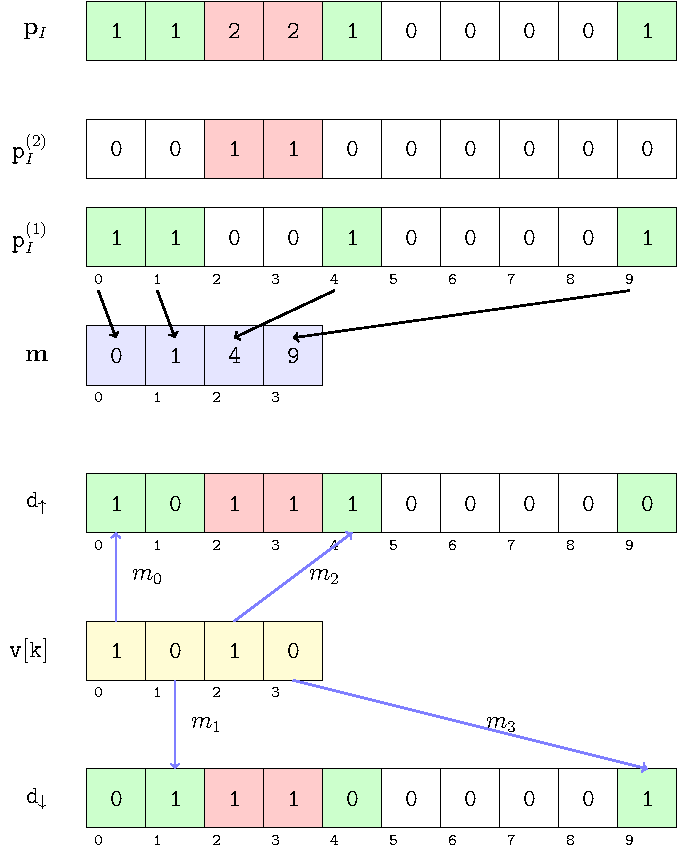
\includegraphics[width=0.9\columnwidth]{pattern.tikz} 
\caption{The {\sop} $\mpv_I$ is encoded as in Eq.~\eqref{eq:sop}. Singly and doubly
occupied orbitals are represented respectively in green and red.
The list of indices $\mathbf{m}$ of the singly occupied orbitals is built (in blue), and this
mapping is re-used to build the determinants from permutations generated by Anderson's algorithm (yellow).}
\label{fig:mapping}
\end{figure}

Figure~\ref{fig:mapping} gives a pictorial description of the data structures used to generate a determinant.
To build a generated determinant $(\md_\up,\md_\dn)$ from a permutation $\tu$, one needs to
\begin{enumerate}
    \item Fill the doubly occupied orbitals by setting both $\md_\up$ and $\md_\dn$
          equal to $\mpp_I^{(2)}$
    \item Iterate over the bits of $\tu$. If the $k$-bit is set to \one{}, set the $m_k$-th orbital of $d_\up$ to \one, otherwise set the $m_k$-th orbital of $d_\dn$ to \one.
\end{enumerate}

\subsection{Further optimizations}

As a first optimization, instead of creating each determinant from the
permutation as shown in Fig.~\ref{fig:mapping}, all the determinants can be
generated iteratively by considering only the orbitals that have changed
from the previously generated determinant.
The integer obtained by $\mathtt{v[k-1]} \oplus \mathtt{v[k]}$ has bits set at
the positions where the bits differ between $\mathtt{v[k-1]}$ and
$\mathtt{v[k]}$. The positions of these bits can be found in a few cycles by
iteratively:
\begin{enumerate}
\item counting the number of trailing zeros
\item setting the least significant {\one} to {\zero} by setting
      $\mathtt{v[k] \gets v \wedge (v-1)}$
\end{enumerate}
until $v[k] = 0$. 

A second optimization is to consider time-reversal symmetry. When $n_\up =
n_\dn$, one can remark that ${\mathtt{v[n_{det}}-1-\mathtt{k]} = \neg \mathtt{v[k]}}$, 
where $\mathtt{n_{det}}$ is the number of determinants
\begin{equation}
\mathtt{n_{det}} = \frac{(n_\up +n_\dn)!}{n_\up! n_\dn!}
\end{equation}
%$\mathtt{v[}2^{n_\up+n_\dn}-1-\mathtt{k]} = \neg \mathtt{v[k]}$.
Hence, it suffices to iterate over the first half of the permutations of Anderson's
algorithm, and generate two determinants per iteration.


%%%%%%%%%%%%%%%%%%%%%%%%%%%%%%%%%%%%%%%%%%%%%%%%%%%%%%%%%%%%%%%%%
\section{Shifted Epstein-Nesbet denominators}
%%%%%%%%%%%%%%%%%%%%%%%%%%%%%%%%%%%%%%%%%%%%%%%%%%%%%%%%%%%%%%%%%


Let us consider a real-valued normalized spin-adapted wave function with
energy $E$, expressed as
\begin{equation}
\ket{\Psi} = \sum_{i \in \mathcal{I}} c_i \ket{D_i}
\end{equation}
which is an eigenfunction of the Hamiltonian projected in the internal space of
determinants $\mathcal{I}$.
The variance of the energy associated with this function is
\begin{equation}
\sigma^2 = \mel{\Psi}{\hat{H}^2}{\Psi} - \mel{\Psi}{\hat{H}}{\Psi}^2 .
\end{equation}
Inserting the resolution of the identity for $\hat{H}^2$ gives an
approximation of the variance truncated to the Full Configuration Interaction
(FCI) space, 
\begin{equation}
\sigma^2 = \sum_{\alpha \in \text{FCI}} \mel{\Psi}{\hat{H}}{\alpha} \mel{\alpha}{\hat{H}}{\Psi} - E^2
\label{eq:ri}
\end{equation}
where $\text{FCI}$ denotes a complete set of arbitrary orthonormal basis
functions, $\ket{\alpha}$, spanning the FCI space.
The FCI space can be split in three subspaces:
\begin{itemize}
\item The internal space $\mathcal{I}$
\item The external space $\mathcal{E}$ which is the subset of functions
      $\ket{\alpha}$ which don't belong to $\mathcal{I}$, and for which
      $\mel{\alpha}{\hat{H}}{\Psi} \ne 0$
\item The rest of the FCI space.
\end{itemize}
$\hat{H}$ is symmetric and $\ket{\Psi}$ is real, so Eq.~\eqref{eq:ri} can be
re-written as
\begin{equation}
\sigma^2 = \sum_{D_i    \in \mathcal{I}} \mel{D_i}{\hat{H}}{\Psi}^2 
         + \sum_{\alpha \in \mathcal{E}} \mel{\alpha}{\hat{H}}{\Psi}^2 - E^2.
\end{equation}
As $\ket{\Psi}$ is an eigenfunction of $\hat{H}$ projected in $\mathcal{I}$, 
\begin{equation}
\mel{D_i}{\hat{H}}{\Psi}^2 = \left( E\, \langle D_i | \Psi \rangle \right)^2 = E^2 c_i^2,
\end{equation}
and as $\ket{\Psi}$ is normalized, one obtains
\begin{equation}
\sigma^2 = \sum_{\alpha \in \mathcal{E}} \mel{\alpha}{\hat{H}}{\Psi}^2.
\end{equation} 

The variance of the energy doesn't depend on the particular choice of the
functions $\ket{\alpha}$, as long as they constitute an orthonormal set of
functions spanning the space $\mathcal{E}$. Moreover, the variance of the
energy is equal for degenerate wave functions with different spin quantum
numbers $m_s$.  Hence, one can choose equivalently the $\ket{\alpha}$'s to be
Slater determinants or \csf s.

The Epstein-Nesbet (EN) second-order perturbative contribution to the energy is given
by
\begin{equation}
\ept = \sum_{\alpha \in \mathcal{E}} \frac{\mel{\alpha}{\hat{H}}{\Psi}^2}{E-\mel{\alpha}{\hat{H}}{\alpha}}.
\label{eq:pt2}
\end{equation}
This equation can be seen as a weighted sum of the different terms involved in
the expression of the variance. However, the weights differ depending on the
choice of $\ket{\alpha}$. Also, when a basis of Slater determinants is chosen,
this expression is not invariant with respect to the choice of $m_s$, and this 
is not desirable.

A way to cure the invariance with respect to $m_s$ is to impose all the weights
to be the same for all the determinants belonging to the same \csf . But as 
the same determinant can appear in the expression of multiple \csf s, Davidson
proposed to use a modified EN zeroth-order Hamiltonian formed from
diagonal elements averaged over Slater determinants belonging to the same
\sop . This idea was implemented 20 years ago in the MELD sCI
program,\cite{Davidson_1979,Kozlowski_1994} and also in SCIEL.\cite{Sciel}

This modified zeroth order Hamiltonian implies that the weight is the same for
all the determinants belonging to the same \sop . This can be done by
inserting a determinant-specific energy shift $\epsilon_\alpha$ to the
diagonal element at the denominator 
\begin{equation}
\ept = \sum_{\alpha \in \mathcal{E}} \frac{\mel{\alpha}{\hat{H}}{\Psi}^2}{E-\left(\mel{\alpha}{\hat{H}}{\alpha}+\epsilon_\alpha \right)}.
\end{equation}
with
\begin{equation}
\epsilon_\alpha = E_\alpha - \mel{\alpha}{\hat{H}}{\alpha} 
\end{equation}
where the shift is chosen to be
\begin{equation}
E_\alpha = \min_{\beta \in \text{\sop}(\alpha)} \mel{\beta}{\hat{H}}{\beta}.
\end{equation}
This choice of $E_\alpha$ is not the same as Davidson's, but it simpler to compute
and gives the same weight for all the values of $m_s$.
Although the generation of all the determinants is extremely fast, using
this approximation can become expensive since it requires to compute
all the diagonal elements $\mel{\beta}{\hat{H}}{\beta}$ for each
$\ket{\alpha}$.

To circumvent this problem, one can remark that for the majority of the
contributions to
\begin{equation}
 \mel{\alpha}{\hat{H}}{\Psi} = \sum_i c_i \mel{\alpha}{\hat{H}}{D_i}
\end{equation}
$\ket{\alpha}$ is doubly excited with respect to $\ket{D_i}$.
We now consider that $\ket{D_i}$ is the determinant with the lowest
energy among all the determinants sharing the same \sop .
For all the other determinants $\ket{D_j}$ belonging to the same \sop{}
as $\ket{D_i}$ and doubly excited with respect to $\ket{D_i}$, one can define
a double excitation operator
\begin{equation}
\hat{T}_{i\rightarrow j} \ket{D_i} = \ket{D_j}.
\end{equation}
Remarking that 
\begin{equation}
\mel{\hat{T}_{i\rightarrow j} D_i}{\hat{H}}{\hat{T}_{i\rightarrow j} \alpha} 
\begin{cases}
\pm \mel{\alpha}{\hat{H}}{D_i} & \text{ if } \hat{T}_{i\rightarrow j}\ket{\alpha} \ne 0 \\
0 & \text{otherwise},
\end{cases}
\end{equation}
the contributions connected by $\hat{H}$ to $\ket{D_j}$ are the
$\hat{T}_{i\rightarrow j} \ket{\alpha}$ which have a diagonal element which
will be shifted by 
\begin{equation}
E_\alpha = \langle \hat{T}_{i\rightarrow j} \alpha | \hat{H} | \hat{T}_{i\rightarrow j} \alpha \rangle - \langle \alpha | \hat{H} | \alpha \rangle
\end{equation}
This quantity may be approximated by
\begin{equation}
E_j = \langle D_j | \hat{H} | D_j \rangle - \langle D_i | \hat{H} | D_i \rangle,
\end{equation}
and the approximate shifts $E_j$ can be precomputed.
If $\ket{\alpha}$ is connected to multiple $\ket{D_i}$, we take the energy
shift associated with the $\ket{D_i}$ with largest associated $|c_i|$.  As our
implementation generates the $\ket{\alpha}$'s with no duplicates from the
$\ket{D_i}$ sorted by decreasing $|c_i|$, the use of the shift can be made at
no cost.





%%%%%%%%%%%%%%%%%%%%%%%%%%%%%%%%%%%%%%%%%%%%%%%%%%%%%%%%%%%%%%%%%
\section{Numerical tests}
%%%%%%%%%%%%%%%%%%%%%%%%%%%%%%%%%%%%%%%%%%%%%%%%%%%%%%%%%%%%%%%%%


%--------------------------------------------
\subsection{Open-shell toy problem}
%--------------------------------------------

To test our implementation with a large number of open shells, we have prepared
model wave functions for the dissociated Chromium dimer in its 13-et state, separated by a
distance of $100$~\AA, using the def2-SVP basis.\cite{Weigend_2005}
At such a large distance, each Chromium atom is in its high-spin state with $6$
unpaired electrons. Two equivalent wave functions are built to initialize the sCI
calculation:
\begin{itemize}
\item The $m_s=6$ wave function, which is a single determinant with $30$ $\up$
      and $18$ $\dn$ electrons.
\item The 13-et $m_s=0$ wave function with $24$ $\up$ and $24$ $\dn$ electrons, which
      contains 924 determinants
\end{itemize}
The system is composed of $62$ molecular orbitals, so for this simple case $\Nint=1$.
The orbitals were obtained at the restricted open-shell Hartree-Fock (ROHF) level
for $m_s=6$.
The selection is performed in the valence Full-CI space, with $20$ frozen electrons.

The $m_s=0$ wave function was initialized by taking the same {\sop} as the
one of the single determinant of the $m_s=6$ wave function, and generating all
the possible determinants using the algorithm presented in this paper.
The generation of the $924$ determinants was done in $\sim 19~200$
CPU cycles ($\sim8$ microseconds), i.e.  $21$~cycles per generated determinant. The Hamiltonian was
diagonalized and we checked that the lowest state with $\langle \stwo \rangle =
42$ had the exact same energy as the $m_s=6$ single determinant.

\begin{figure}
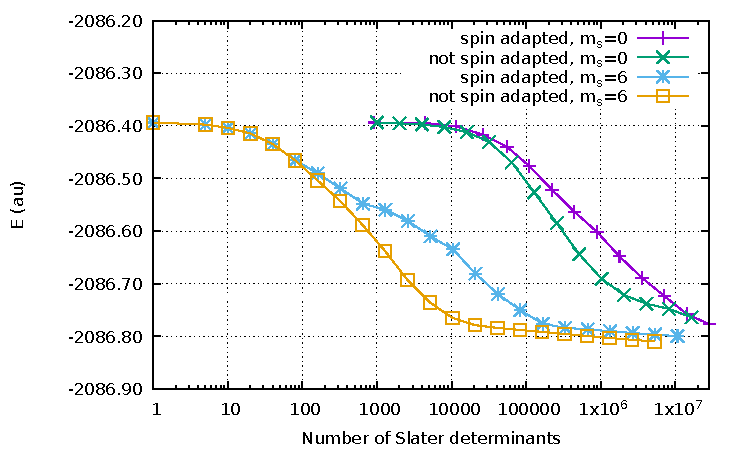
\includegraphics[width=0.9\columnwidth]{e_var_ndet}
\caption{Variational energy of dissociated Cr$_2$ as a function of the number of
selected Slater determinants in the wave function expansion.}
\label{fig:e_var_ndet}
\end{figure}

\begin{figure}
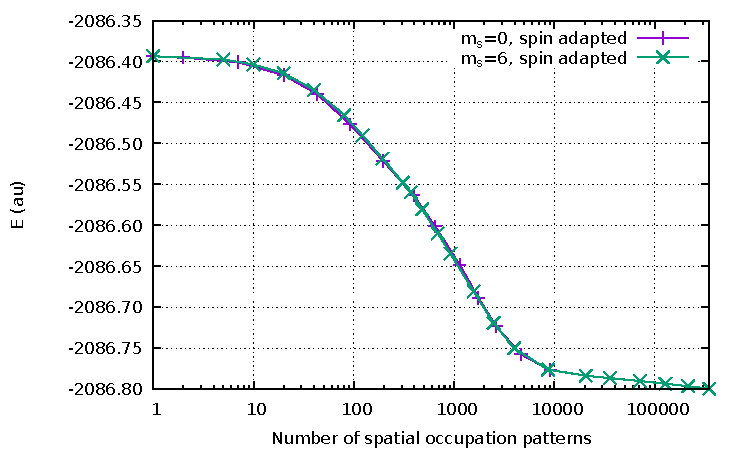
\includegraphics[width=0.9\columnwidth]{e_var_nsop}
\caption{Variational energy of dissociated Cr$_2$ as a function of the number of
selected \sop{}.}
\label{fig:e_var_nsop}
\end{figure}

\begin{figure}
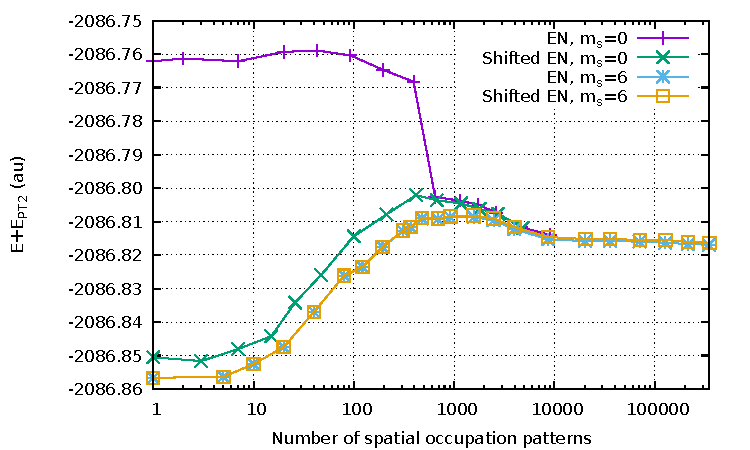
\includegraphics[width=0.9\columnwidth]{e_pt2_nsop}
\caption{Variational energy with second order perturbative correction of
dissociated Cr$_2$ as a function of the number of selected \sop{}, using
the EN denominators or the shifted EN denominators.}
\label{fig:e_pt2_nsop}
\end{figure}

For the $m_s=6$ wave function, we have run a CIPSI selection imposing or not the
wave function to be spin-adapted. As expected, for the same energy the number of
determinants is increased when spin adaptation is imposed. Then, we have run the
CIPSI selection for the $m_s=0$ wave function imposing the
spin adaptation. The convergence of the energy is plotted as a function of the
number of determinants in Fig.~\ref{fig:e_var_ndet}, and as a function of
the number of \sop{} in Fig.~\ref{fig:e_var_nsop}.
From Fig.~\ref{fig:e_var_nsop}, it is striking that the $m_s=0$ and $m_s=6$
wave functions are indeed equivalent.
This example exhibits the fact that having a large number of determinants with
small weights is not always characteristic of a multi-reference character.
Moreover, the number of determinants is not a relevant criterion for the
quality of a wave function, as opposed to \csf s. However, using \sop s
appears as a cheap alternative to \csf s when working in the determinant
framework.

Fig.~\ref{fig:e_pt2_nsop} shows that the EN $\ept$ values are very different
between $m_s=6$ and $m_s=0$ when the number of \sop{} is less than 1000. The
shifted EN and the EN values give almost identical energy curves for $m_s=6$.
%The tiny difference comes from the slightly different selection of determinants
%induced by the change of perturbation expression.
On the contrary, the shifted EN
corrects the wrong behavior of the curve for small numbers of \sop{}, and then
the shifted EN and the EN curves join, before converging to the same curve as
the $m_s=6$ curve. When the shifted EN and EN curves join, it is the sign
that all the determinants of the external space with low energies were included
in the internal space. In addition, the $E$ term in the denominator becomes more
negative as plotted in Fig.~\ref{fig:e_var_nsop}, so all the denominators tend to be large enough so that the use of the energetic shift becomes less and
less important.


%--------------------------------------------
\subsection{Avoided crossing of LiF}
%--------------------------------------------

The avoided crossing between the ionic and neutral $^1\Sigma^+$ states of LiF is a 
common benchmark for correlated methods, as the location of the crossing is highly
sensitive to the amount of correlation. At large distances, the lowest triplet state
is very close in energy to the singlet states. If the wave function is not
spin adapted, the triplet state will mix with the singlets during the selection
and the convergence of the CIPSI calculations to the correct states is not guaranteed.

\begin{figure}
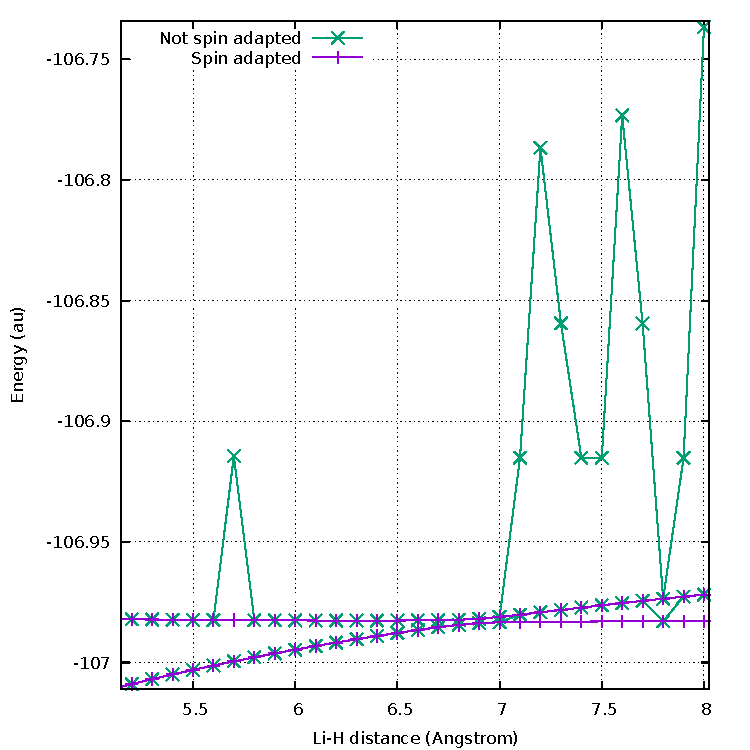
\includegraphics[width=0.9\columnwidth]{lif}
\caption{Avoided crossing of LiF, with and without imposing spin adaptation.}
\label{fig:lif}
\end{figure}

To show the importance of spin adaptation for such a problem, we have reported
in Fig.~\ref{fig:lif} the potential energy curve of the two lowest states of
LiF computed with and without imposing spin adaptation. For all the distances,
the CIPSI calculations were run blindly (with no user interaction), starting
with the CAS-SCF(2,2)/aug-cc-pVDZ  wave functions of both states (four
determinants). Only the lowest molecular orbital was frozen, corresponding to
the $1s$ orbital of the Fluorine atom. The calculations were stopped when the
second-order perturbative contribution was below $0.1$~m$E_h$ or when the
number of determinants reached 4 million.

Fig.~\ref{fig:lif} shows that for large distances, without spin adaptation
there are multiple erratic points for which the two obtained states are not
the desired ones. This curve also shows that all the points obtained with spin
adaptation converged to the correct states.

%--------------------------------------------
\subsection{Adiabatic transition energy of formaldehyde}
%--------------------------------------------

The last example we present is the calculation of the adiabatic transition
energy of the formaldehyde molecule with the aug-cc-pVDZ basis set.  The ground
state is well described by a single determinant, and the excited state is an
open shell singlet obtained by a $^1(n \rightarrow \pi^*)$ single excitation,
so its main {\csf} contains two determinants.  The geometries of the ground and
excited states were taken from Ref~\citep{Loos_2018}. For both geometries, a
preliminary CIPSI calculation was run to produce state-averaged natural
orbitals, in order to produce molecular orbitals of comparable quality for
both states. Hence, the rate of convergence of the energy with respect to the
number of selected \csf s is expected to be comparable for both states.
However, we expect the rate of convergence of the energy with respect to the
number of selected determinants to be different. 

For each state a state-specific CIPSI calculation was run at its equilibrium
geometry.
For the excited state, the run was initiated using a wave function with
the two determinants of the reference \csf , and a state-following approach was
used during the Davidson diagonalization to avoid collapsing to the ground state.

The qualitative difference between the two states (single determinant
\textit{vs} open-shell singlet) makes the computation of
the energy difference inaccurate if the energy difference is calculated for
the same number of selected determinants. 
However, one can compute the energy difference for the same number of selected
\sop, which is expected to be consistent with the use of the same number of
\csf s.

\begin{figure}
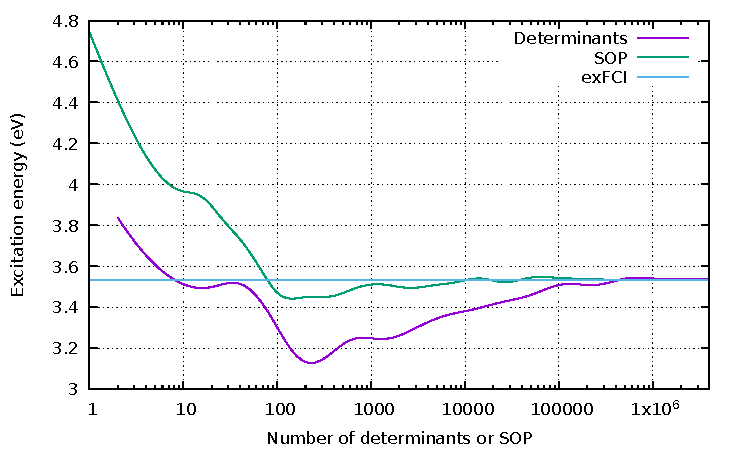
\includegraphics[width=0.9\columnwidth]{formaldehyde}
\caption{Adiabatic transition energy of formaldehyde, computed with fixed numbers of 
determinants and fixed numbers of \sop .}
\label{fig:formaldehyde}
\end{figure}

Figure~\ref{fig:formaldehyde} plots the adiabatic transition energy computed
taking the energies of both states with the same number of selected
determinants, and taking the energies of both states with the same number of
\sop{}.
As the two runs were independent, the number of selected determinants and
\sop s were different for the two states so a cubic spline interpolation
was used to compute the energies at arbitrary numbers of determinants.
This figure shows that the adiabatic transition energy converges much
faster to 3.53~eV using the \sop{} criterion, a value close to the
experimental value of 3.50~eV.\cite{Clouthier_1983,Angeli_2005}

%TODO : montrer ndet/nsop

%%%%%%%%%%%%%%%%%%%%%%%%%%%%%%%%%%%%%%%%%%%%%%%%%%%%%%%%%%%%%%%%%
\section{Conclusion}
%%%%%%%%%%%%%%%%%%%%%%%%%%%%%%%%%%%%%%%%%%%%%%%%%%%%%%%%%%%%%%%%%

We have presented a general algorithm to complement an arbitrary wave function
with all the required Slater determinants to obtain eigenstates of the $\stwo$
operator when the Hamiltonian is diagonalized, in a negligible time.  This
spin adaptation is done after the selection of determinants in the selected CI
algorithm.
The presented examples have illustrated different situations where
spin adaptation is important.  When comparing wave functions, considering the
number of \csf s is more relevant than the number of Slater determinants and
considering \sop s allows to stay in the determinant framework while still
benefiting from the consistence brought by \csf s.
Finally, we would like to emphasize that this spin adaptation procedure can be
applied to any selected CI method : Heat-Bath CI, Machine Learning CI, Monte
Carlo CI, \textit{etc}.

%%%%%%%%%%%%%%%%%%%%%%%%%%%%%%%%%%%%%%%%%%%%%%%%%%%%%%%%%%%%%%%%%

\begin{acknowledgments}
The authors gratefully acknowledge Sean Eron Anderson for creating the 
\emph{Bit Twiddling Hacks} web page.
This work was performed using HPC resources from CALMIP (Toulouse) under
allocation 2018-0510 and from GENCI-TGCC (Grant 2018-A0040801738).
KG acknowledges support from grant number CHE1762337 from the U.S. National Science Foundation.
\end{acknowledgments}

%%%%%%%%%%%%%%%%%%%%%%%%%%%%%%%%%%%%%%%%%%%%%%%%%%%%%%%%%%%%%%%%%

\bibliography{s2}

\end{document}
